%%%%%%%%%%%%%%%%%%%%%%%%%%%%%%%%%%%%%%%%%
% Beamer Presentation
% LaTeX Template
% Version 1.0 (10/11/12)
%
% This template has been downloaded from:
% http://www.LaTeXTemplates.com
%
% License:
% CC BY-NC-SA 3.0 (http://creativecommons.org/licenses/by-nc-sa/3.0/)
%
%%%%%%%%%%%%%%%%%%%%%%%%%%%%%%%%%%%%%%%%%

%----------------------------------------------------------------------------------------
%	PACKAGES AND THEMES
%----------------------------------------------------------------------------------------

\documentclass{beamer}

\mode<presentation> {

% The Beamer class comes with a number of default slide themes
% which change the colors and layouts of slides. Below this is a list
% of all the themes, uncomment each in turn to see what they look like.

%\usetheme{default}
%\usetheme{AnnArbor}
%\usetheme{Antibes}
%\usetheme{Bergen}
%\usetheme{Berkeley}
%\usetheme{Berlin}
%\usetheme{Boadilla}
%\usetheme{CambridgeUS}
%\usetheme{Copenhagen}
%\usetheme{Darmstadt}
%\usetheme{Dresden}
%\usetheme{Frankfurt}
%\usetheme{Goettingen}
%\usetheme{Hannover}
%\usetheme{Ilmenau}
%\usetheme{JuanLesPins}
%\usetheme{Luebeck}
\usetheme{Madrid}
%\usetheme{Malmoe}
%\usetheme{Marburg}
%\usetheme{Montpellier}
%\usetheme{PaloAlto}
%\usetheme{Pittsburgh}
%\usetheme{Rochester}
%\usetheme{Singapore}
%\usetheme{Szeged}
%\usetheme{Warsaw}

% As well as themes, the Beamer class has a number of color themes
% for any slide theme. Uncomment each of these in turn to see how it
% changes the colors of your current slide theme.

%\usecolortheme{albatross}
%\usecolortheme{beaver}
%\usecolortheme{beetle}
%\usecolortheme{crane}
%\usecolortheme{dolphin}
%\usecolortheme{dove}
%\usecolortheme{fly}
%\usecolortheme{lily}
%\usecolortheme{orchid}
%\usecolortheme{rose}
%\usecolortheme{seagull}
%\usecolortheme{seahorse}
%\usecolortheme{whale}
%\usecolortheme{wolverine}

%\setbeamertemplate{footline} % To remove the footer line in all slides uncomment this line
%\setbeamertemplate{footline}[page number] % To replace the footer line in all slides with a simple slide count uncomment this line

%\setbeamertemplate{navigation symbols}{} % To remove the navigation symbols from the bottom of all slides uncomment this line
}

\usepackage{graphicx} % Allows including images
\usepackage{booktabs} % Allows the use of \toprule, \midrule and \bottomrule in tables

%----------------------------------------------------------------------------------------
%	TITLE PAGE
%----------------------------------------------------------------------------------------

\title[Docker (An opinionated guide)]{Docker (An opinionated guide)} % The short title appears at the bottom of every slide, the full title is only on the title page

\author{Alexander Morton} % Your name
\institute[Financial Cloud] % Your institution as it will appear on the bottom of every slide, may be shorthand to save space
{
Financial Cloud\\ % Your institution for the title page
\medskip
\textit{alex.morton@financial-cloud.com} % Your email address
}
\date{\today} % Date, can be changed to a custom date

\begin{document}

\begin{frame}
\titlepage % Print the title page as the first slide
\end{frame}

\begin{frame}
\frametitle{Overview} % Table of contents slide, comment this block out to remove it
\tableofcontents % Throughout your presentation, if you choose to use \section{} and \subsection{} commands, these will automatically be printed on this slide as an overview of your presentation
\end{frame}

%----------------------------------------------------------------------------------------
%	PRESENTATION SLIDES
%----------------------------------------------------------------------------------------

%------------------------------------------------
\section{Introduction} % Sections can be created in order to organize your presentation into discrete blocks, all sections and subsections are automatically printed in the table of contents as an overview of the talk
%------------------------------------------------

\subsection{What's the problem?} 
\begin{frame}
    \frametitle{What's the problem?}
    \textit{My application needs this file/binary/environment/application to run. Shouldn't take you long to install...}
    \begin{itemize}
        \item Things to consider about the application itself
        \begin{itemize}
            \item What version do you need?
            \item Does it run in a particular version of a certain OS?
            \item What does it need access to?
            \item What access rights does it need?
            \item Does all of the above affect other components of your applications?
            \item Does this need to communicate with the outside world?
        \end{itemize}
    \end{itemize}
    \begin{itemize}
        \item Things to consider about production and development
        \begin{itemize}
            \item \textbf{You will usually need to have some development version}
            \item Will you have to consider your cloud provider's requirements in addition to your own?
            \item Do you need to reconfigure the full application to safely test it?
        \end{itemize}
    \end{itemize}
\end{frame}

\subsection{What's the solution?} 

\begin{frame}
\frametitle{What's the solution?}
\small
\textbf{There is never just one solution}
\begin{itemize}
    \item Virtual machines have there place if you need a single OS which is completely isolated.
    \item You may also not want to use the docker engine.
    \item Cloud provider allow you to more easily setup virtual machines. \textit{The Amazon Machine Image (AMI) would be an example}
\end{itemize}
\begin{figure}
    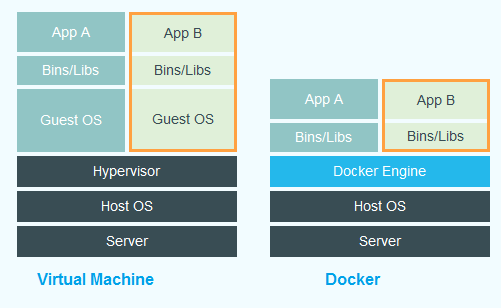
\includegraphics[scale=0.40]{./pics/container_vs_vm.png}
    \caption{You have two options to this problem}
\end{figure}
\end{frame}

%------------------------------------------------
\subsection{Docker solution} 
\begin{frame}
    \frametitle{Docker solution}
    \small
    "Docker is a computer program that performs operating-system-level virtualization also known as containerization." \tiny \cite{dockerwiki}
    \small
    \vspace{5mm}
    \begin{columns}
    \column{0.7\textwidth}
    \textbf{Basically we use features of the linux kernel \tiny \cite{dockeroverview}}
    \small
    \begin{itemize}
        \item \textbf{Namespaces}: Processes only see resources associated to there namespace.
        \item \textbf{CGroups}: Processes use of resources are isolated into groups.
    \end{itemize}
    \textbf{What this allows you to do}
    \begin{itemize}
        \item Build your application state in layers. If you change a layer then all previous layers taken directly from cache. \textbf{Faster builds}
        \item Only build your application with the stuff it needs. \textbf{More efficient when running \tiny \cite{justefficient}}
    \end{itemize}
    \column{0.3\textwidth}
    \begin{figure}
    
\includegraphics[scale=0.3]{./pics/docker.png}
    \caption{\tiny Docker is nothing more than a bunch of containers on top of a whale [Whale, 2018]}
    \end{figure}
    \end{columns}
    \vspace{1mm}
\tiny
"Docker is the company driving the container movement and the only container platform provider to address every application across the hybrid cloud."\cite{whatisdocker}
\end{frame}

%------------------------------------------------
\section{How to use docker}
\subsection{Docker file commands} 
\begin{frame}
Creating an image can be done with a handful of commands. \tiny \cite{dockerinstructions} 
\small
\frametitle{Docker File Commands}
\begin{block}{FROM}
This instruction is used to set the base image for subsequent instructions. It is mandatory to set this in the first line of a Dockerfile. You can use it any number of times though.
\end{block}

\begin{block}{MAINTAINER}
This is a non-executable instruction used to indicate the author of the Dockerfile.
\end{block}

\begin{block}{RUN}
This instruction lets you execute a command on top of an existing layer and create a new layer with the results of command execution.
\end{block}

\end{frame}
\begin{frame}
\small
\begin{block}{CMD}
The major difference between CMD and RUN is that CMD doesn’t execute anything during the build time. It just specifies the intended command for the image. Whereas RUN actually executes the command during build time.
\end{block}

\begin{block}{EXPOSE}
While running your service in the container you may want your container to listen on specified ports. 
\end{block}

\begin{block}{COPY/ADD}
This instruction is used to copy files and directories from a specified source to a destination (in the file system of the container).
ADD is the same but allows remote urls.
\end{block}

\begin{block}{ENTRYPOINT}
You can use this instruction to set the primary command for the image.
\end{block}

\end{frame}
\begin{frame}
\small
\begin{block}{VOLUME}
You can use the VOLUME instruction to enable access to a location on the host system from a container. Just pass the path of the location to be accessed.
\end{block}

\begin{block}{USER}
This is used to set the UID (or username) to use when running the image.
\end{block}
\begin{block}{WORKDIR}
This is used to set the currently active directory for other instructions such as RUN, CMD, ENTRYPOINT, COPY and ADD.
\end{block}

\begin{block}{ONBUILD}
This instruction adds a trigger instruction to be executed when the image is used as the base for some other image. It behaves as if a RUN instruction is inserted immediately after the FROM instruction of the downstream Dockerfile.
\end{block}

\end{frame}

%----------------------------------------------
\subsection{Example docker file} 
\begin{frame}[fragile] 
\frametitle{Example docker file}
\begin{example}[Base Image for all ours apps in production]
\tiny
\begin{verbatim}
FROM node:carbon

# Set working directory for container
ENV HOME=/usr/app/nodeApp
WORKDIR $HOME

# Need to install aws-cli so the container can get the environment file on startup.
RUN apt-get update
RUN apt-get install -qq -y python-pip libpython-dev 
RUN curl -O https://bootstrap.pypa.io/get-pip.py
RUN python get-pip.py
RUN pip install awscli

# Install vim for development
RUN apt-get install vim -y

RUN mkdir -p $HOME
RUN mkdir -p $HOME/logs

# Give everyone including node user the ability to execute/read/write to app directory.
# Need to write to app so we can run startup script.
RUN chmod -R o+rwx /usr/app/nodeApp 

COPY ./.aws $HOME/.aws
RUN aws s3 cp s3://npmrc/.npmrc ./.npmrc

RUN npm i -g pm2
COPY ./setup.sh $HOME
\end{verbatim}
\end{example}
\begin{example}[We expand on that base image for each app]
\tiny
\begin{verbatim}
FROM 000000000.dkr.ecr.eu-west-3.amazonaws.com/production-base:latest

COPY ./package.json $HOME/
COPY ./dist $HOME/dist/
COPY ./UI/dist $HOME/UI/dist/

ENV NODE_ENV=production
RUN npm install

ENV JSON=rules-engine.json

# Setup will get env file and set VPC dependent env variables.
CMD ["bash","/usr/app/nodeApp/setup.sh"]
\end{verbatim}
\end{example}
\end{frame}


\begin{frame}[fragile] 
\frametitle{Example docker file}
\begin{example}[We expand on that base image for each app]
\tiny
\begin{verbatim}
FROM 0000000000.dkr.ecr.eu-west-3.amazonaws.com/production-env:latest

COPY ./package.json $HOME/
COPY ./dist $HOME/dist/
COPY ./UI/dist $HOME/UI/dist/

ENV NODE_ENV=production
RUN npm install

ENV JSON=rules-engine.json

# Setup will get env file and set VPC dependent env variables.
CMD ["bash","/usr/app/nodeApp/setup.sh"]
\end{verbatim}
\end{example}
\end{frame}

%------------------------------------------------
\subsection{Docker CLI} 
\begin{frame}
    \small
    \frametitle{Docker CLI}
    \textbf{Now we have a docker file what do we do next?}
    \begin{itemize}
        \item Install docker
        \begin{itemize}
            \item  Easy for mac and linux. Windows is another story
        \end{itemize}
        \item Pull in other peoples images to base your project on
        \item Build your own image from the base image
        \item Run the image
        \begin{itemize}
            \item  A running image is the container.
            \item You can then access most containers with a bash shell.
        \end{itemize}
    \end{itemize}
    \begin{figure}
    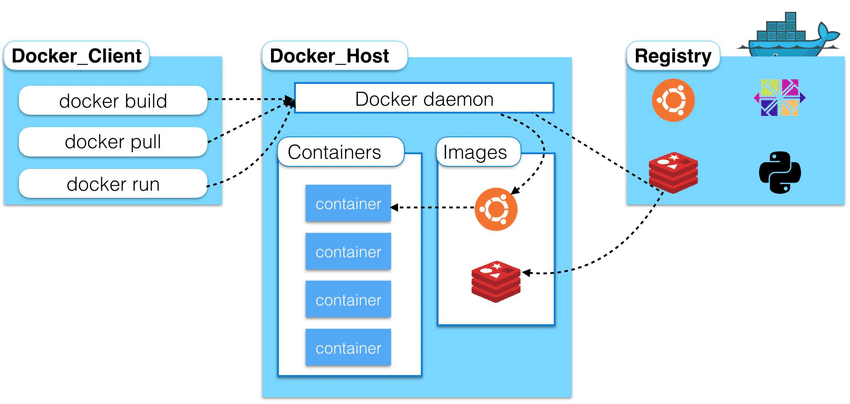
\includegraphics[scale=0.25]{./pics/High-level-overview-of-Docker-architecture.jpg}
    \end{figure}
\end{frame}

\section{Conclusion} 
\begin{frame}
    \small
    \frametitle{Conclusion}
    \begin{itemize}
        \item Lots of videos/blogs on the subject
        \item Docker is a useful tool for the novice and the tech genius
        \item Containerization underpins many leading edge technologies
        \begin{itemize}
            \item AWS Fargate and serverless lambdas are two example we use here
        \end{itemize}    
        \item Docker Rivals
        \begin{itemize}
            \item Don't confuse container orchestration and container engine
            \item If you interested in docker alternatives rkt is one which works with kubernetes.
            \item Don't forget VM still have a place.
        \end{itemize}
        \item Even if you don't use containers in production they can make development a lot easier
        \item We haven't even touched on container orchestration and networking    
    \end{itemize}    
\end{frame}

%------------------------------------------------

\begin{frame}
\frametitle{References}
\footnotesize{
\begin{thebibliography}{99} % Beamer does not support BibTeX so references must be inserted manually as below
\bibitem[Docker, 2018]{whatisdocker} Docker (2018)
\newblock What is Docker
\newblock \href{https://www.docker.com/what-docker}{https://www.docker.com/what-docker} 

\bibitem[Docker Wiki, 2018]{dockerwiki} Docker Wiki (2018)
\newblock Docker Wiki
\newblock \href{https://en.wikipedia.org/wiki/Docker_(software)}{https://en.wikipedia.org/wiki/Docker\_(software)} 

\bibitem[Container Journal, 2016]{justefficient} Container Journal (2018)
\newblock Docker: Not Faster than VMs, but More Efficient
\newblock \href{https://containerjournal.com/2016/11/21/docker-not-faster-vms-just-efficient/}{https://containerjournal.com/2016/11/21/docker-not-faster-vms-just-efficient/} 

\bibitem[Docker Overview, 2016]{dockeroverview} Docker Overview (2016)
\newblock What Is Docker? How Does It Work?
\newblock \href{https://devopscube.com/what-is-docker/}{https://devopscube.com/what-is-docker/} 

\bibitem[Dockerfile Instructions and Syntax, 2015]{dockerinstructions} Dockerfile Instructions and Syntax (2015)
\newblock Dockerfile Instructions and Syntax
\newblock \href{https://deis.com/blog/2015/dockerfile-instructions-syntax/}{https://deis.com/blog/2015/dockerfile-instructions-syntax/} 

\end{thebibliography}
}
\end{frame}

%------------------------------------------------

\begin{frame}
\Huge{\centerline{The End}}
\end{frame}

%----------------------------------------------------------------------------------------

\end{document}